\documentclass[10pt,compress,handout]{beamer}
    \useoutertheme{miniframes}
    \usepackage[english]{babel}
    %\usepackage[margin=1in]{geometry}

    \usepackage{amsmath}
    \usepackage{amsfonts} 
    \usepackage{amssymb}
    \usepackage{amsthm}
    \usepackage{mathtools}

    \usepackage[utf8]{inputenc}
    %\usepackage[exscale, amsfonts, amssymb]{concmath}
    %\renewcommand*{\bfseries}{\mdseries}

    \usepackage{float}
    \usepackage{graphicx}
    \usepackage{caption}
    \usepackage{subcaption}

    \graphicspath{{./src/figures/}}

    %\usepackage{fancyhdr} %custom headers and footers layout
    \usepackage{lastpage} %package to print the last page
    %\pagestyle{fancy} %fancy page style

    \usepackage{textcomp} 
    \usepackage{multicol} 
    \usepackage{multirow}

    \usepackage[table]{xcolor}
    \usepackage{booktabs}

    \usepackage[backend=biber,
    bibstyle=ieee, 
    citestyle=numeric-comp,
    natbib=true,
    doi=false, 
    url=false,
    isbn=false,
    mincitenames=1,
    maxcitenames=1,
    minbibnames=1,
    maxbibnames=99,
    backref=false,]
    {biblatex}
    \addbibresource[label=main]{./src/references.bib}

    \usepackage{url}
    \usepackage{hyperref}

    %edit the properties of your PDF documents which will be displayed
    \hypersetup{
        bookmarks=true, 		% show bookmarks bar?
        unicode=true,  		% non-Latin characters in Acrobat’s bookmarks
        pdftoolbar=true,        % show Acrobat’s toolbar?
        pdfmenubar=true,        % show Acrobat’s menu?
        pdffitwindow=true,      % page fit to window when opened
        pdftitle={EIS --- Basics},    % title
        pdfauthor={M. Skocic},     % author
        pdfsubject={},   % subject of the document
        pdfnewwindow=true,      % links in new window
        pdfkeywords={}, % list of keywords
        colorlinks=false,       % false: boxed links; true: colored links
        linkcolor=red,          % color of internal links
        citecolor=green,        % color of links to bibliography
        filecolor=magenta,      % color of file links
        urlcolor=cyan           % color of external links
    }

    \usepackage{tikz}
    \usepackage{circuitikz}
    \usetikzlibrary{decorations.pathmorphing,arrows,calc}

    \title{Electrochemical Impedance Spectroscopy for Corrosion}
    \author{M. Skocic, PhD Electrochemistry and Materials}
    \date{\vfill 
\includegraphics[width=0.70\textwidth]{full_bw.png}}   

    \setlength{\parskip}{6pt}
    \newcommand{\coef}{1}

\begin{document}
    \begin{frame}
        \titlepage
    \end{frame}

    \begin{frame}
        \frametitle{Contents}
        \tableofcontents
    \end{frame}
    
\section{Introduction}
    \begin{frame}{Introduction}
        There are 2 categories of electrochemical techniques: 
        time domain and frequency domain \citep{bard2001}.

        Time domain :
        \begin{itemize}
            \item Voltammetry: $I=f(U)$.
            \item Chronoamperometry: $\Delta U$, $I(t)$.
            \item Zero Resistance Ammeter: $\int j_{gal} \cdot dt$.
            \item \ldots
        \end{itemize}

        Frequency domain:
        \begin{itemize}
            \item Electrochemical Impedance Spectroscopy: EIS.
            \item PhotoElectrochemical Impedance Spectroscopy: PEIS.
        \end{itemize}

        Advantages of EIS:
        \begin{itemize}
            \item Measurement in small perturbations (linearization).
            \item Different processes have different time constants.
            \item Large frequency range from $\mu Hz$ to $GHz$.
        \end{itemize}
    \end{frame}

\section{Basics}
    \subsection{What is EIS?}
    \begin{frame}{Black Box Approach}
        Assume a black box with terminals.

        One applies a voltage and measures the current response (or vice versa).

        Periodic signal with an angular frequency $\omega = 2\pi f$
        with $0 \le \omega < \infty$:
        \begin{itemize}
            \item Voltage $V(\omega) = V_0 e^{j \omega t}$  
            \item Voltage $I(\omega) = I_0 e^{j \omega t - \Phi}$  
        \end{itemize}
        
        \begin{columns}
            \centering
            \column{0.3\textwidth}\centering
                \begin{figure}[h]
                    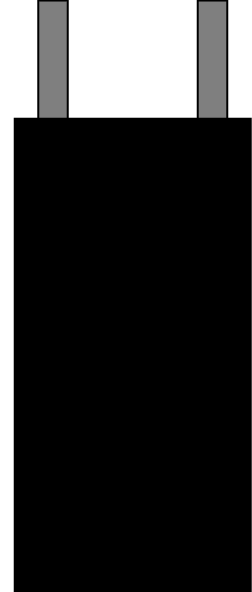
\includegraphics[width=0.5\textwidth]{EIS-black_box}
                \end{figure}
            \column{0.35\textwidth}\centering
                \begin{figure}
                    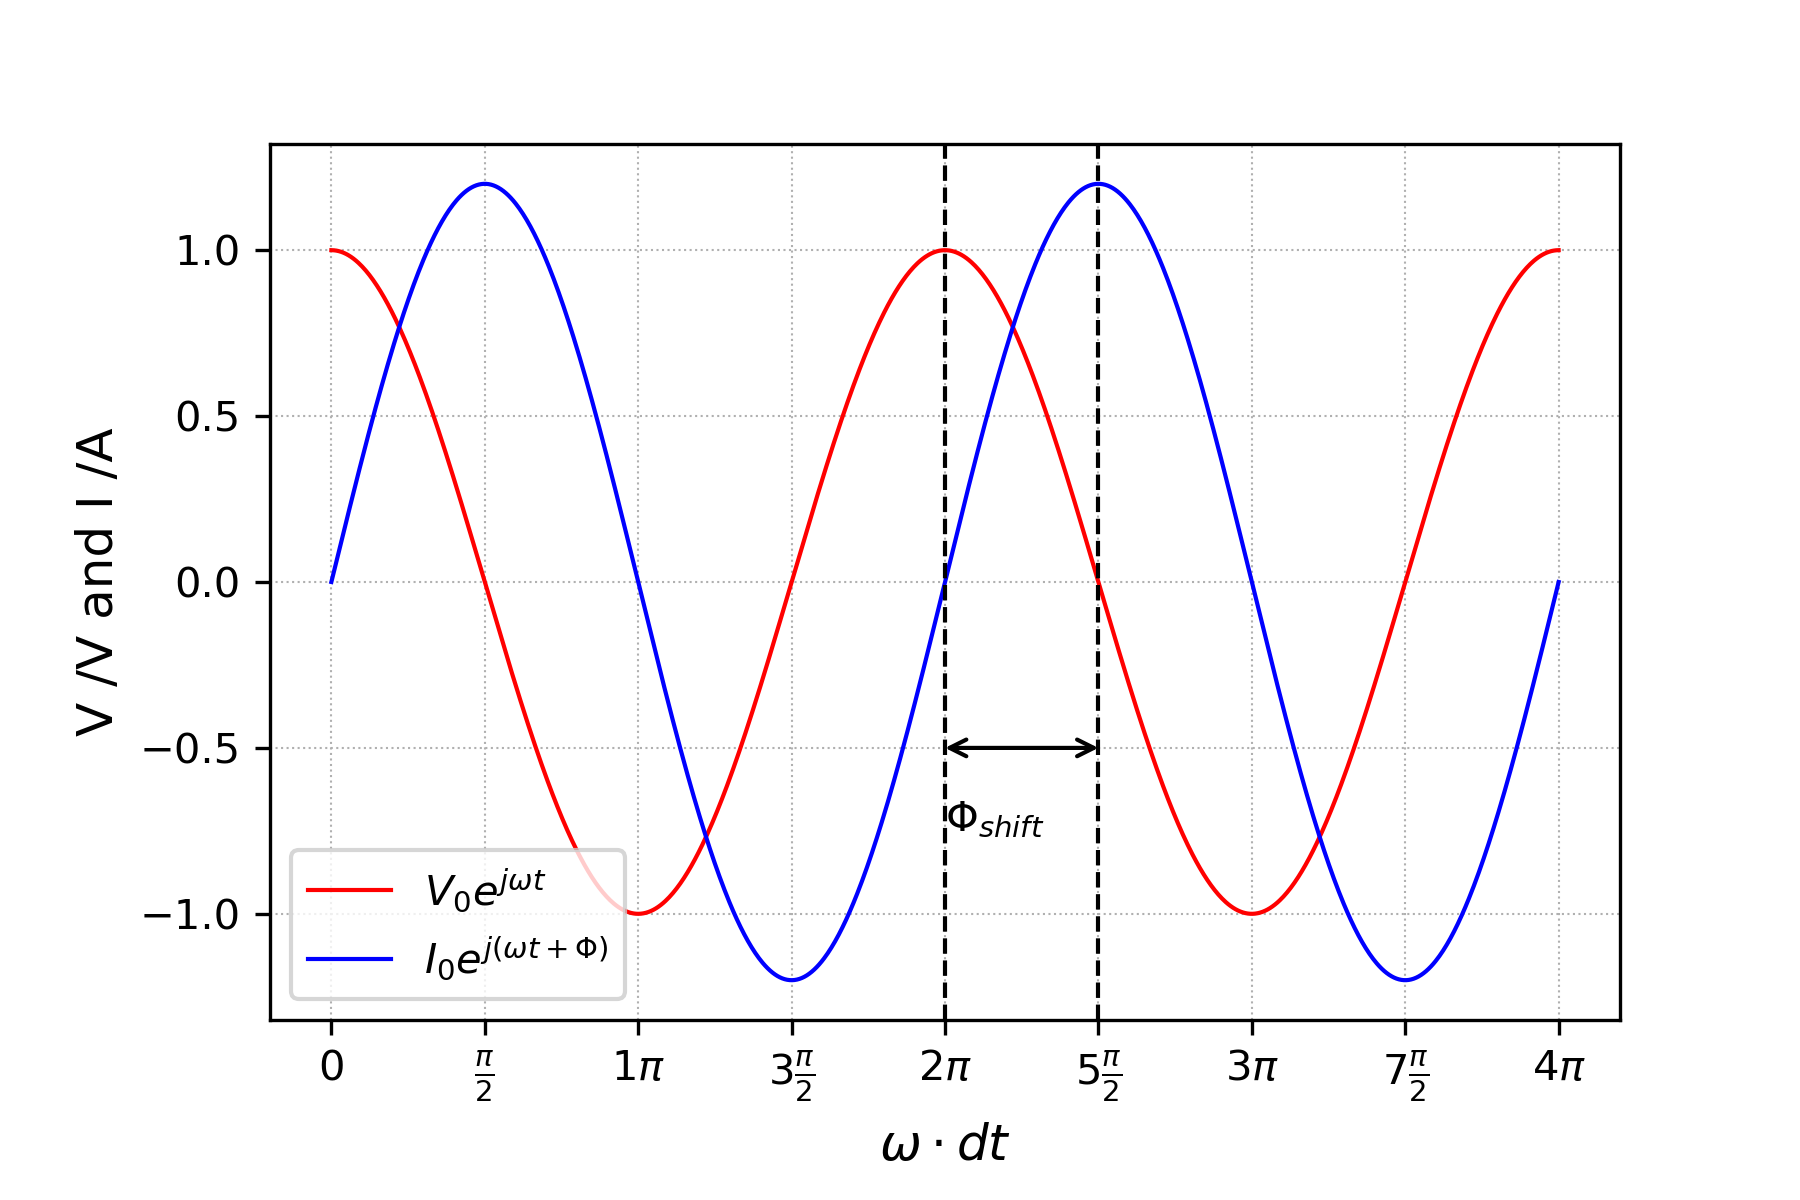
\includegraphics[width=\textwidth]{EIS-ac_waves}
                \end{figure}
            \column{0.35\textwidth}\centering
                \begin{figure}
                    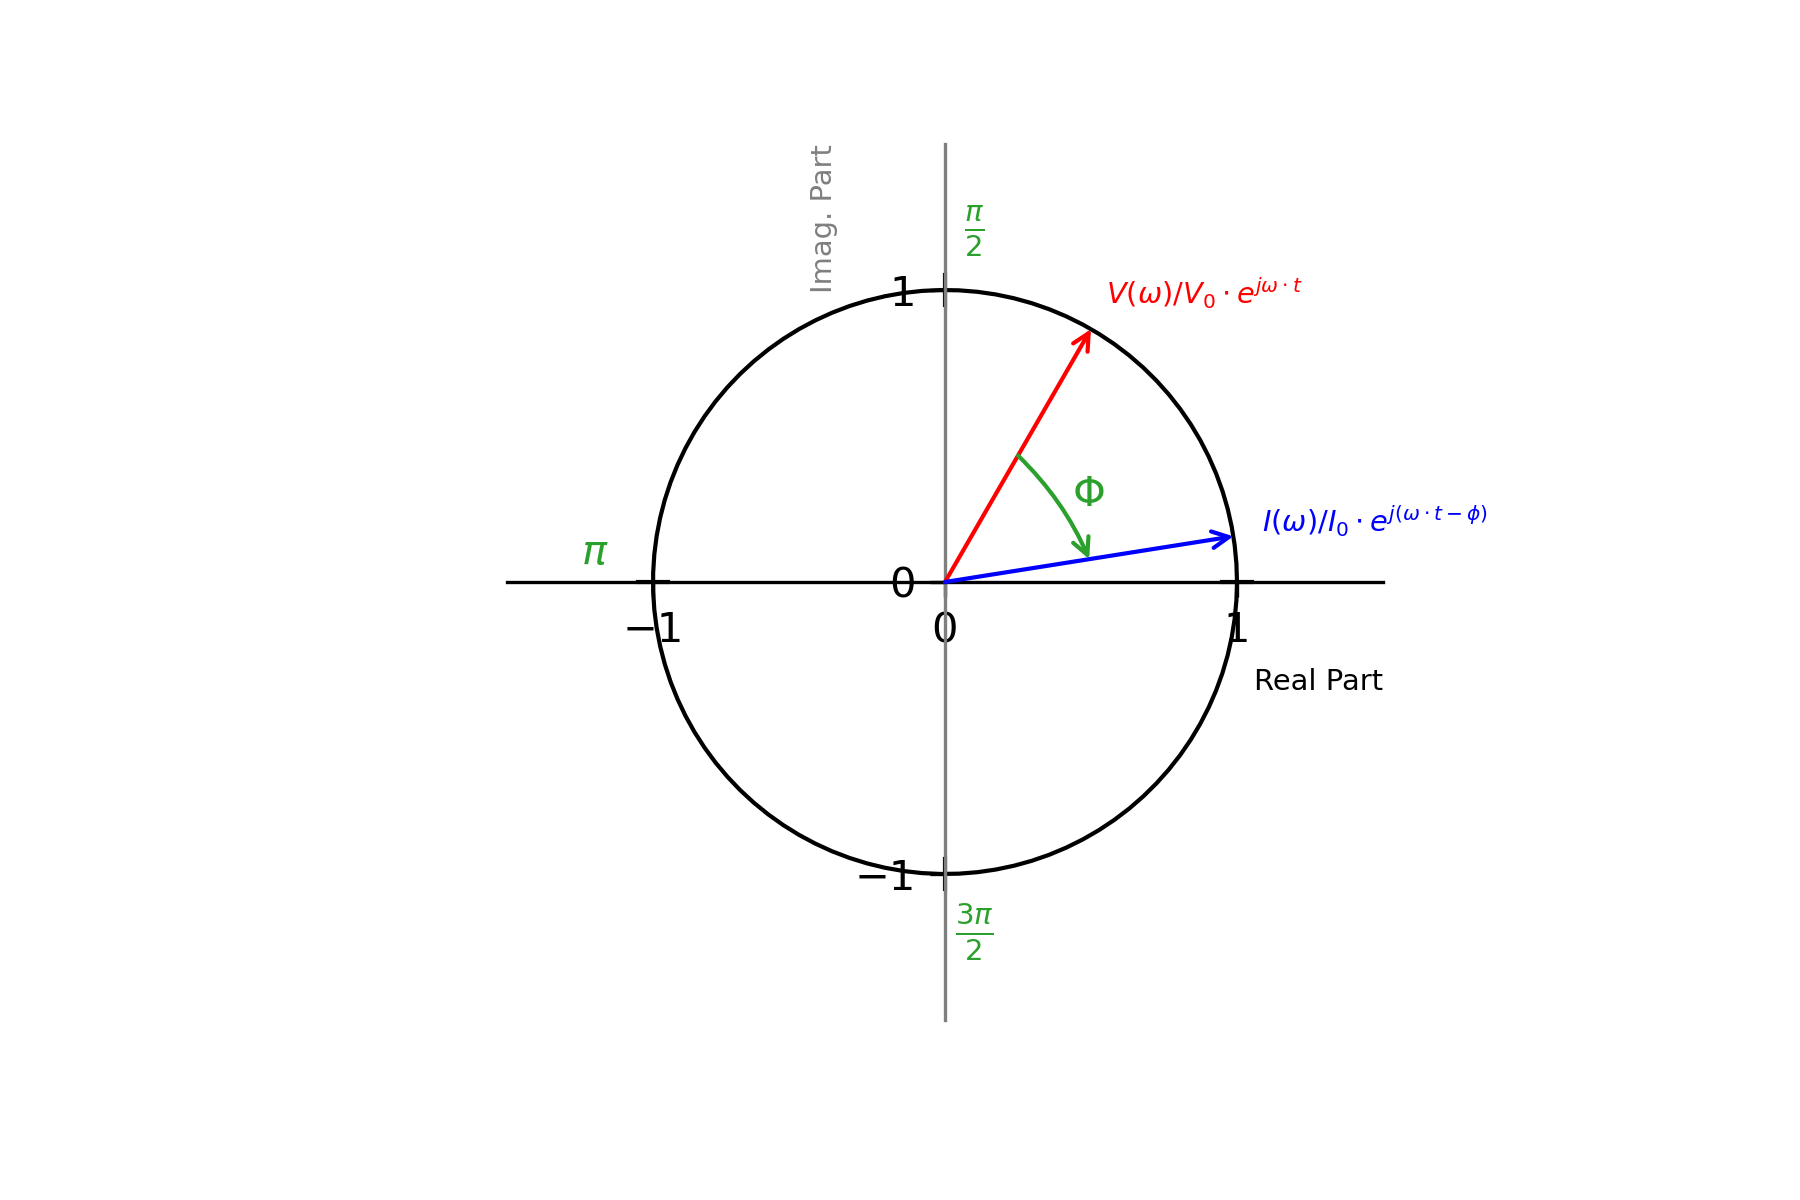
\includegraphics[width=1.3\textwidth]{EIS-ac_waves-trigcircle}
                \end{figure}
        \end{columns}
    \end{frame}
    
    \begin{frame}{Complex Impedance}
        The complex impedance is determined from the imposed voltage/current and the measured
        current/voltage through the Ohm's law:
        $$ Z(\omega) = \frac{V(\omega)}{I(\omega)} = \frac{V_0}{I_0} e^{j \Phi} = Z_0 e^{j\Phi}$$

        Therefore:
        \begin{itemize}
            \item  resistive behavior: $ReZ=Z_0 \cdot \cos \Phi$
            \item  capacitive/inductive behavior $ImZ=Z_0 \cdot \sin \Phi$
        \end{itemize}
        
        Sometimes, the complex admittance $Y(\omega)$ can also be used which is defined as the inverse of the
        complex impedance $Z(\omega)$ 
        $$Y(\omega)=\frac{1}{Z(\omega)}$$
    \end{frame}

    \subsection{Visualization}
    \begin{frame}[allowframebreaks=1.0]{Representations}
        The impedance $Z(\omega)$ can be represented in two different ways:
        \begin{itemize}
            \item  Nyquist plot: represents the real and imaginary parts of $Z(\omega)$ using cartesian coordinates.
            \item  Bode plot: shows the phase shift and magnitude changes in the rang of applied frequencies.
        \end{itemize}
    
        The Bode plot has great advantages for observing phase changes. 
        Therefore, it is useful for the study of sensors, filters, and transistors in electronic devices.
        
        The Nyquist plot provides a better insight into the possible mechanisms.

        \framebreak
        Among these two types of representations, the Nyquist plot is more often used to analyze the characteristics of
        electrochemical processes occurring during corrosion.
        \begin{columns}
            \centering
            \column{0.33\textwidth}
                \centering
                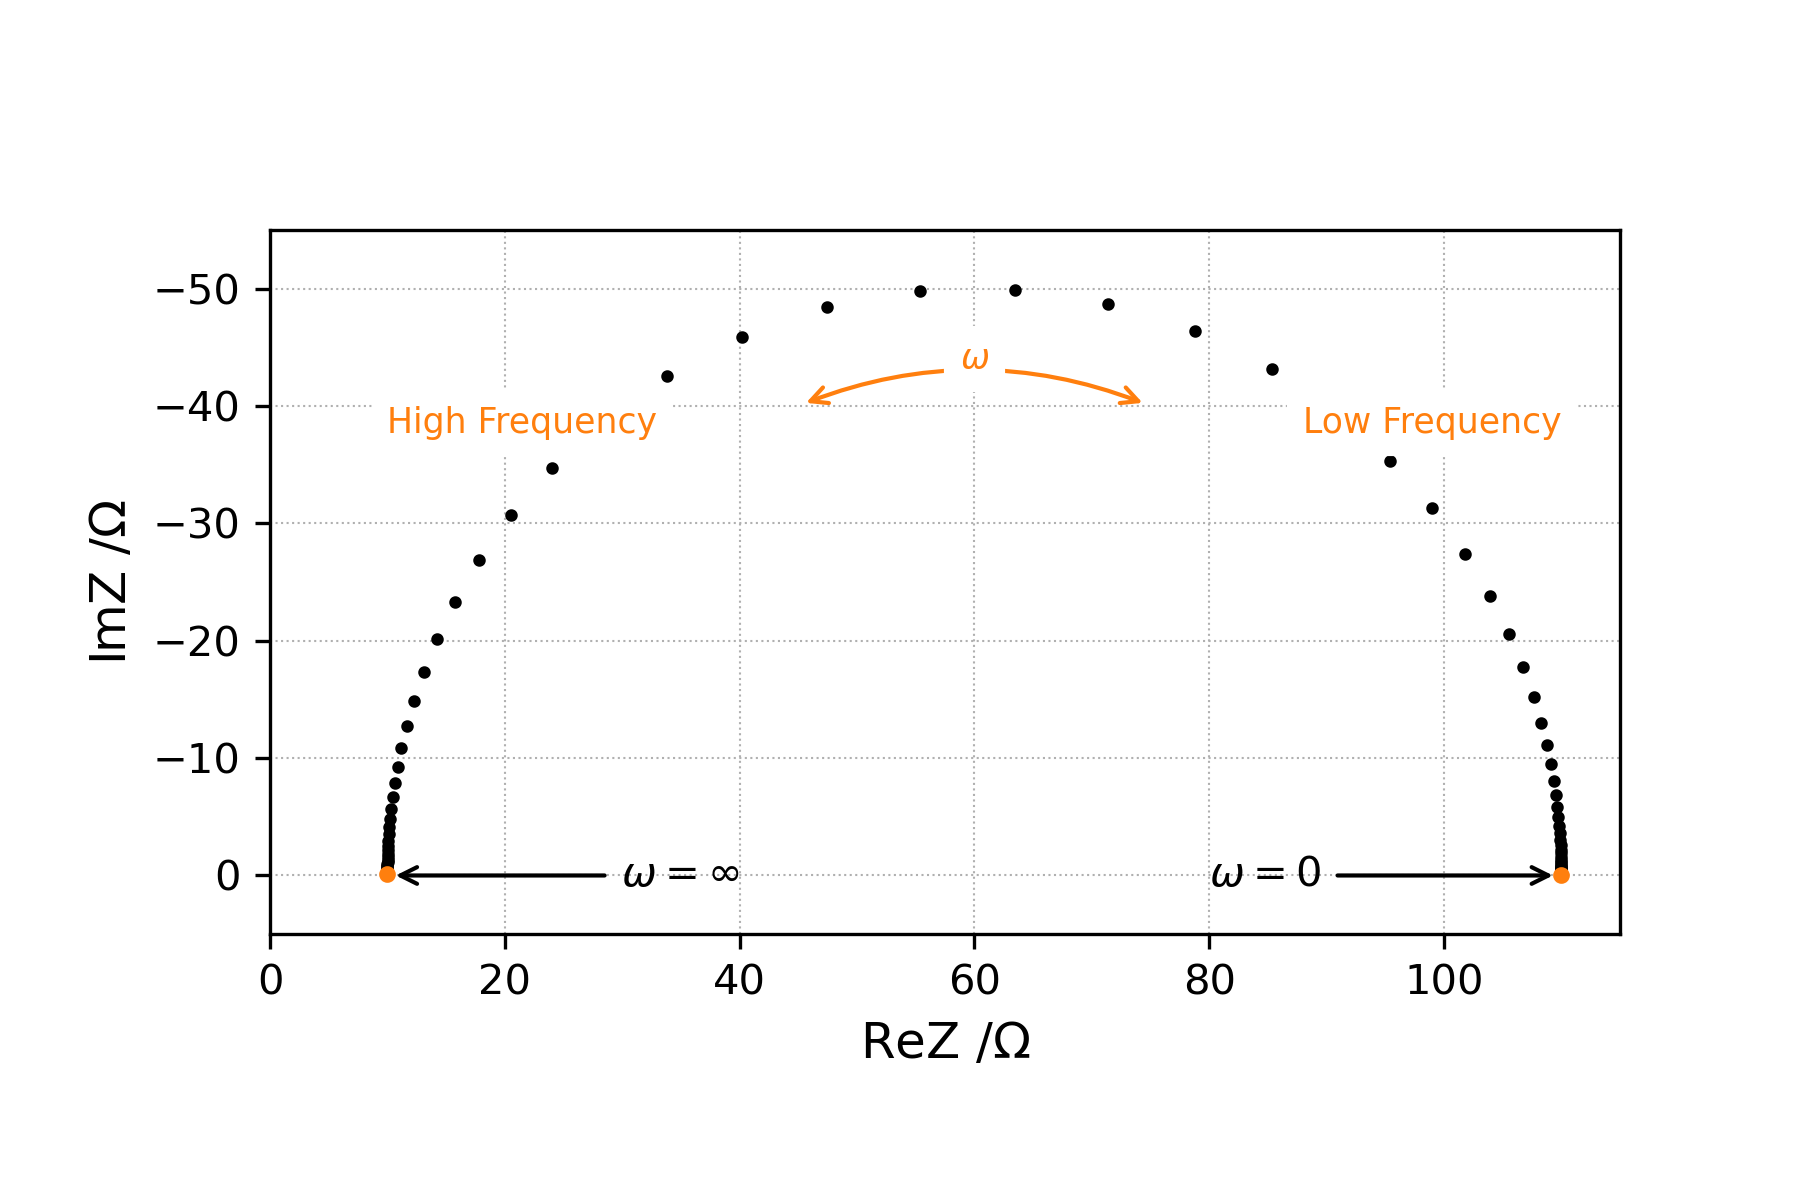
\includegraphics[width=\textwidth]{EIS-example-np}
                Nyquist Plot
            \column{0.33\textwidth}
                \centering
                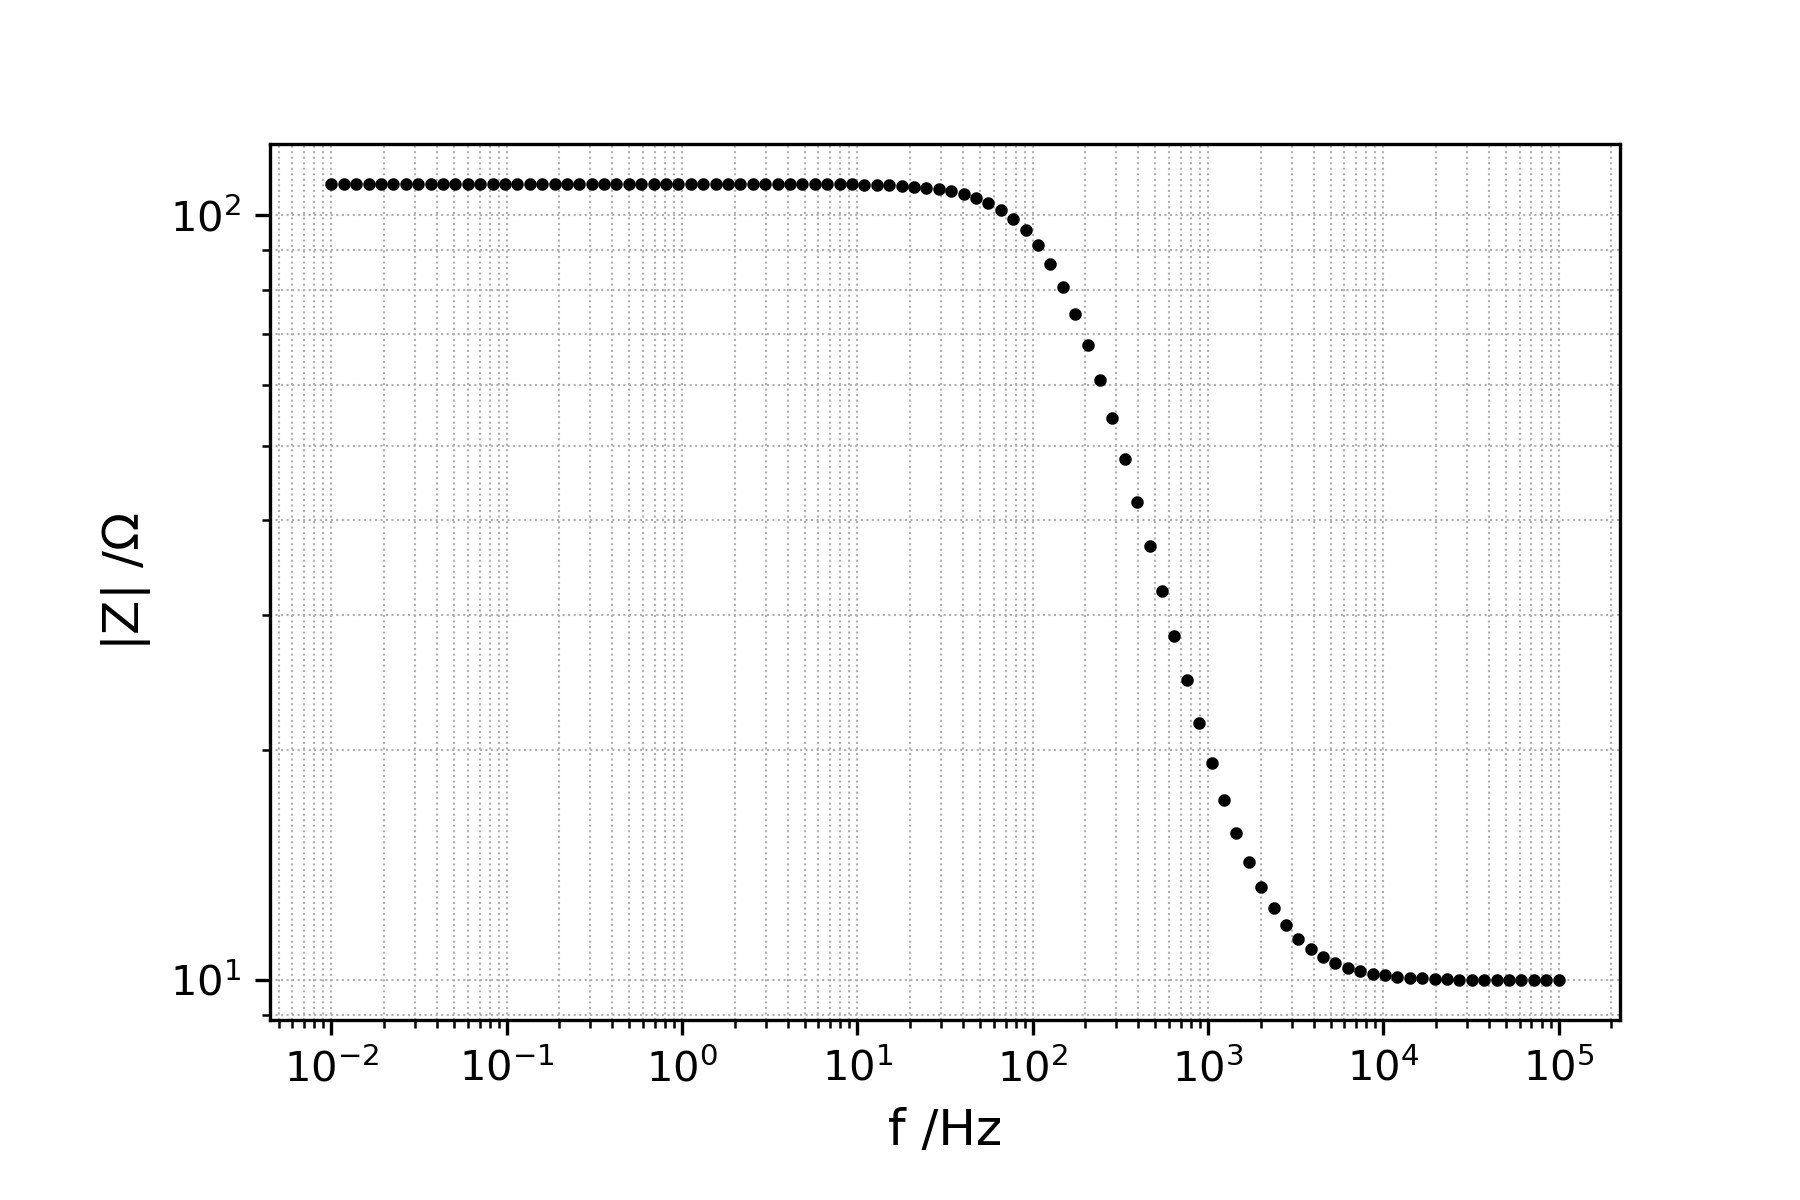
\includegraphics[width=\textwidth]{EIS-example-bm}
                Bode Plot - Magnitude
            \column{0.33\textwidth}
                \centering
                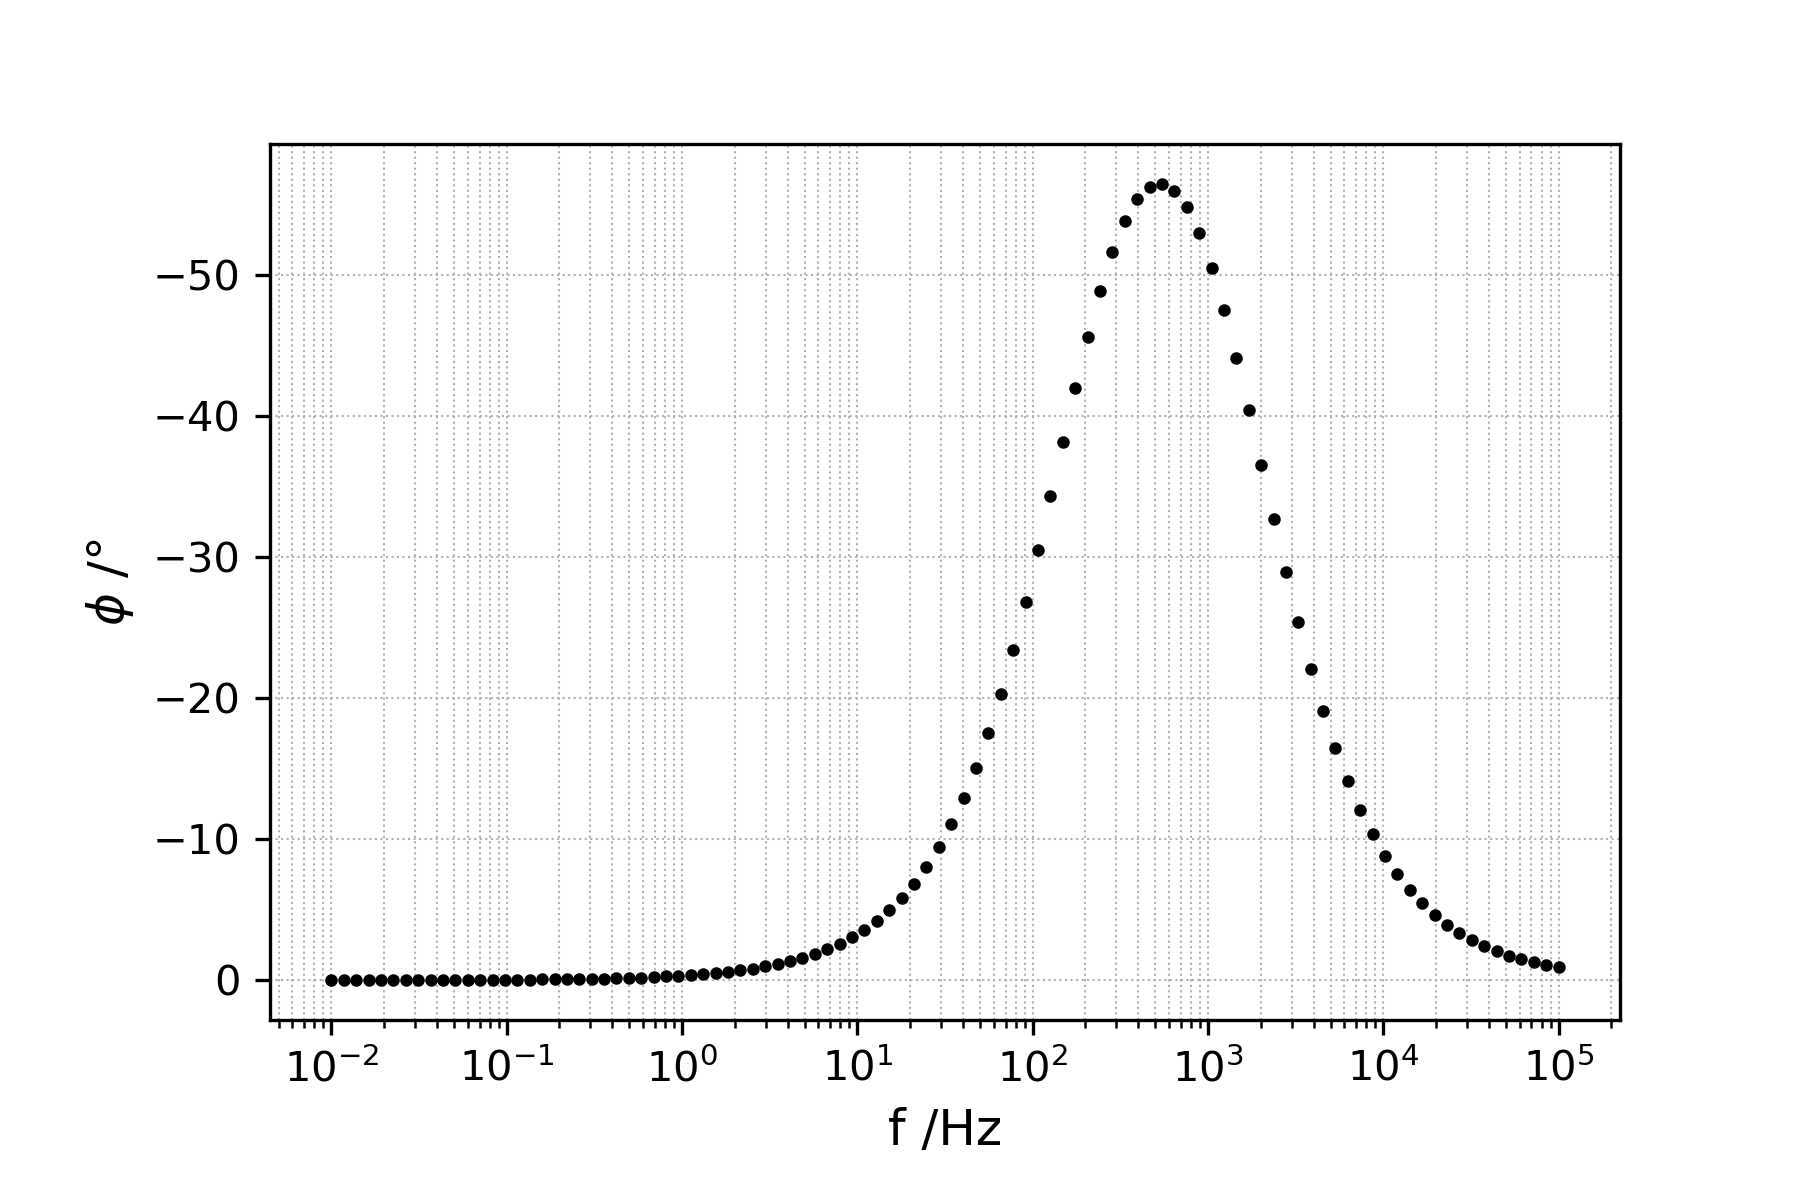
\includegraphics[width=\textwidth]{EIS-example-bp}
                Bode Plot - Phase
        \end{columns}
    \end{frame}
    
    \subsection{Connections}
    \begin{frame}{Series and parallel connections}
        Series connections: $Z_1$ --- $Z_2$ --- \ldots --- $Z_n$
        $$ Z_{eq} = \sum _{i=1}^n Z_i $$

        Parallel connections: $Z_1$ / $Z_2$ / \ldots / $Z_n$ 
        $$ \frac{1}{Z_{eq}} = \sum _{i+1}^n \frac{1}{Z_i} $$
        $$ Z_{eq} = \left( \sum _{i=1}^n \frac{1}{Z_i} \right)^{-1} $$
    \end{frame}

    \subsection{Equivalent Circuits}
    \begin{frame}{Equivalent Circuit Models}
        The circuit model for EIS consists of a combination of electrical circuit elements\citep{orazem2008}:
        \begin{itemize}
            \item ideal elements:
            \begin{itemize}
                \item  resistors (R)
                \item  capacitors (C)
                \item inductors (L)
            \end{itemize}
            \item nonideal capacitor-like element: Constant Phase Element (CPE or Q)
            \item diffusion elements:
            \begin{itemize}
                \item semi-infinite Warburg (W)
                \item finite length warburg ($W_{\delta}$ or O or FLW)
                \item finite space warburg ($W_m$ or T or FSW)
            \end{itemize}
        \end{itemize}
        The circuit model represents the entire system.
    
        The aim is to build an optimal circuit model that is physically meaningful and minimizes the
        number of variables \citep{boukamp1986}.
    \end{frame}

    \begin{frame}{Circuit Elements}
        \begin{columns}
            \column{0.5\textwidth}
                $R$ (Resistor): $Z(\omega)=R$ 

                $C$ (Capacitor): $Z(\omega)=\frac{1}{jC\omega}$

                $L$ (Inductor): $Z(\omega)=jL\omega$

                $Q$ (CPE\footnotemark[4]): $Z(\omega)=\frac{1}{Q(j\omega)^{\alpha}}$

                $W$ (SIW\footnotemark[1]): $Z(\omega)=\frac{\sigma}{\sqrt{\omega}} \cdot (1-j)$
                
                $W_{\delta}$ (FLW\footnotemark[2]): $Z(\omega)=\frac{R_{\delta} \cdot \tanh \sqrt{j\omega\tau}}{\sqrt{j\omega\tau}}$
                
                $W_m$ (FSW\footnotemark[3]): $Z(\omega)=\frac{R_{m} \cdot \coth \sqrt{j\omega\tau}}{\sqrt{j\omega\tau}}$
            \column{0.5\textwidth}
                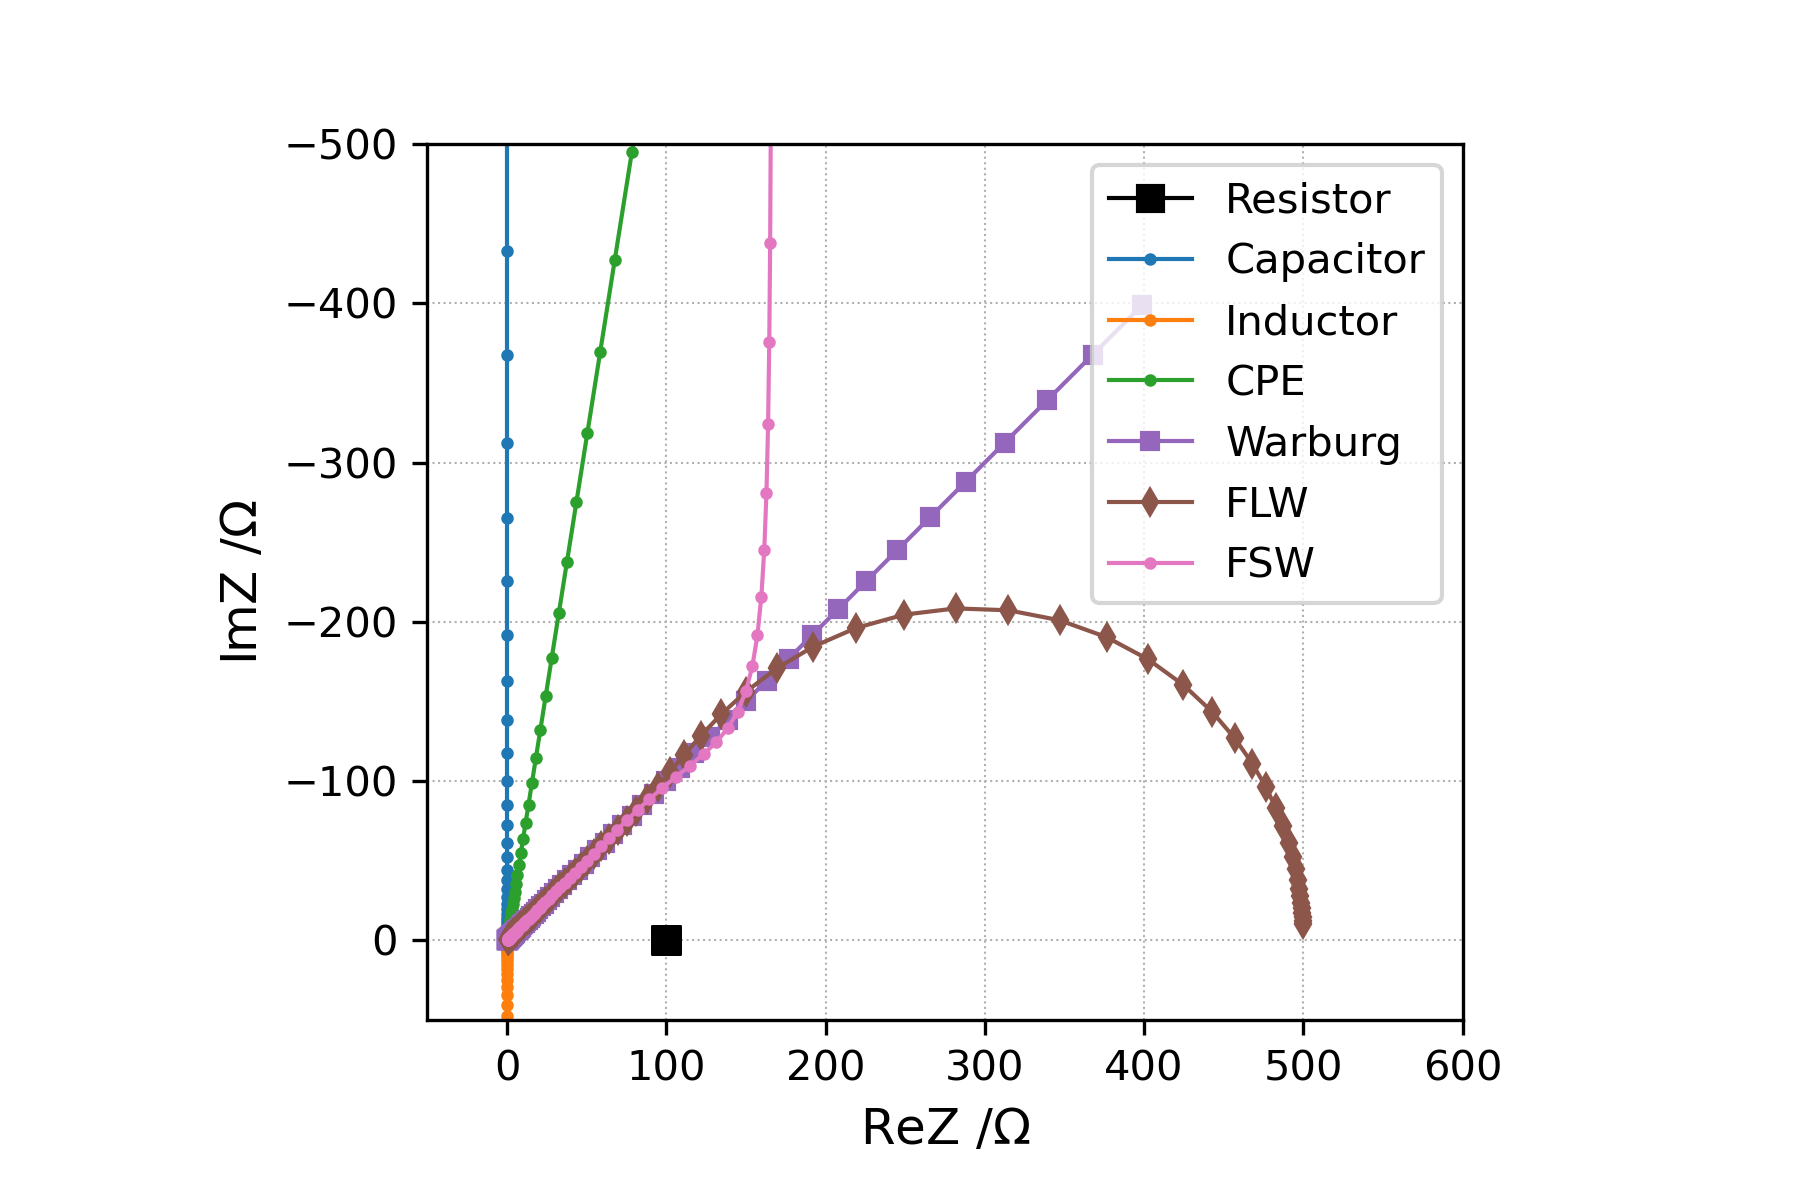
\includegraphics[width=0.5\paperwidth]{EIS-example-np_circuit_elements}
        \end{columns}
        \footnotetext[1]{SIW = Semi-Infinite Warburg}
        \footnotetext[2]{FLW = Finite Length Warburg}
        \footnotetext[3]{FSW = Finite Space Warburg}
        \footnotetext[4]{CPE = Constant Phase Element}
    \end{frame}
    
    \subsection{Physical Parameters}
    \begin{frame}{Circuit Elements and Physical Parameters}
        \begin{columns}[t]
            \column{0.7\textwidth}
                Resistors can be linked to resistivity or kinetics \citep{barsoukov2005}\\
                $R = \rho \cdot \frac{\delta}{A}$ \\
                $R = \frac{RT}{FAj_0(\alpha _a + \alpha _c)} = \frac{RT}{AF^2k^0K_c (\alpha _a + \alpha _c)}$\\[0.25cm]

                Capacitors can be linked to layer thickness: \\
                $C = \frac{\epsilon \epsilon _0 A}{\delta}$\\[0.25cm]

                Warburg elements can be linked to diffusion\\
                $\sigma = \frac{RT}{Az^2F^2\sqrt{2}} \cdot \left( \frac{1}{\sqrt{D}C^*_O} + \frac{1}{\sqrt{D}C^*_R} \right)$\\
                $R = \frac{RT}{Az^2F^2\sqrt{2}} \cdot \frac{\delta}{DC^*}$\\
                $\tau = \frac{\delta ^2}{D}$\\[0.25cm]

                Coupling with other electrochemical techniques helps for determining all 
                necessary parameters.
            \column{0.3\textwidth}{\tiny
                $R$: resistance [$\Omega$]

                $\rho$: resistivity [$\Omega \cdot m$]
                
                $\delta$: thickness [$m$]
                
                $A$: Area [$m^2$]
                
                $j_0$: exchange current density [$A \cdot m^{-2}$]
                
                $k^0$: kinetics constant [$m \cdot s^{-1}$]
                
                $\alpha _a$: anodic transfer coefficient 
                
                $\alpha _c$: cathodic transfer coefficient 
                
                $\epsilon$: relative permittivity
                
                $\epsilon _0$: vaccum permittivity [$F \cdot m^{-1}$]
                
                $C^*$: bulk concentration [$mol \cdot m^{-3}$]

            }
        \end{columns}
    \end{frame}
    
    \subsection{Examples}
    \begin{frame}{Simplified Randles Circuit}
        Reflects an electrochemical reaction controlled only by kinetics \citep{lazanas2023}.

        $R_{el}$: electrolyte resistance

        $R_ct$: charge transfer resistance

        $C_{dl}$: double layer capacitance

        \begin{columns}
            \column{0.5\textwidth}
                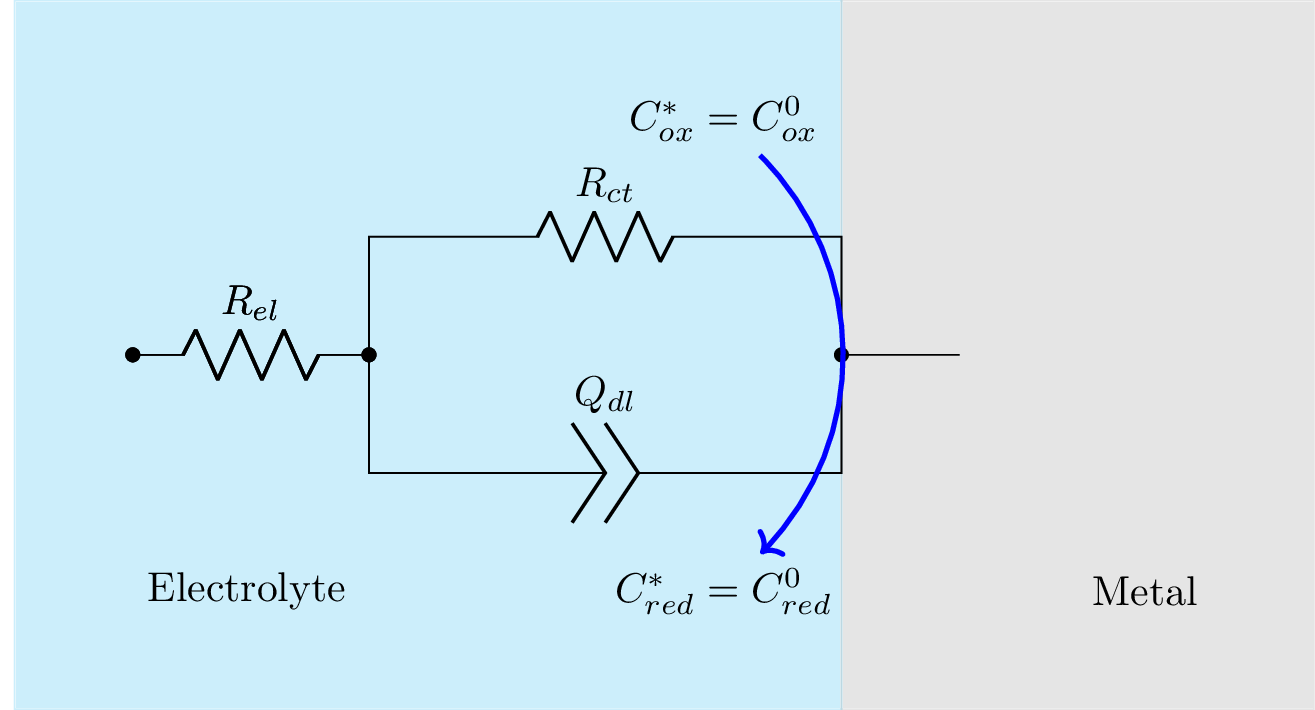
\includegraphics[width=\textwidth]{EIS-circuit-simple_randles}
            \column{0.5\textwidth}
                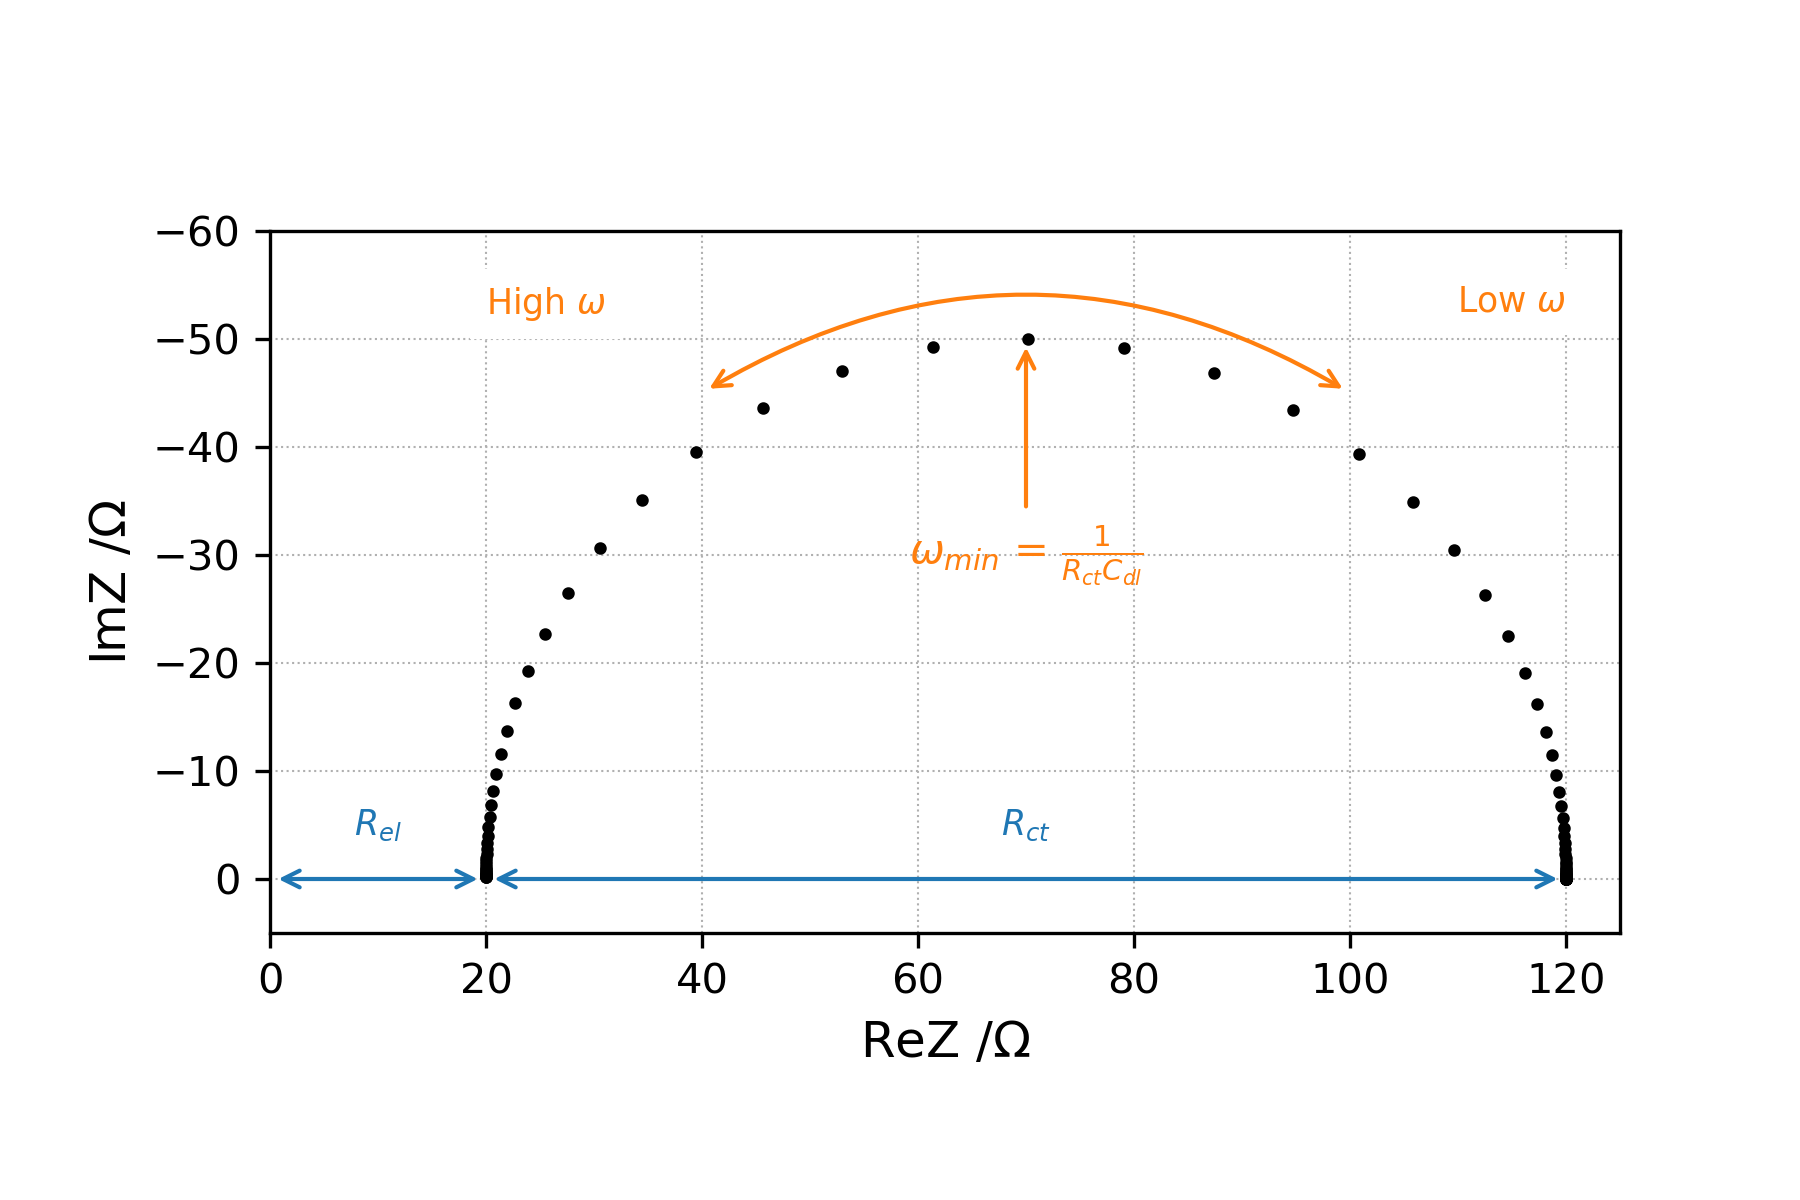
\includegraphics[width=\textwidth]{EIS-example-simple_randles}
        \end{columns}
    \end{frame}

    \begin{frame}{Randles Circuit}
        Reflects electrochemical reaction controlled by kinetics and diffusion \citep{lazanas2023}.

        $R_{el}$: electrolyte resistance

        $R_{ct}$: charge transfer resistance

        $C_{dl}$: double layer capacitance

        $W$: semi-infinite diffusion
        \begin{columns}
            \column{0.5\textwidth}
                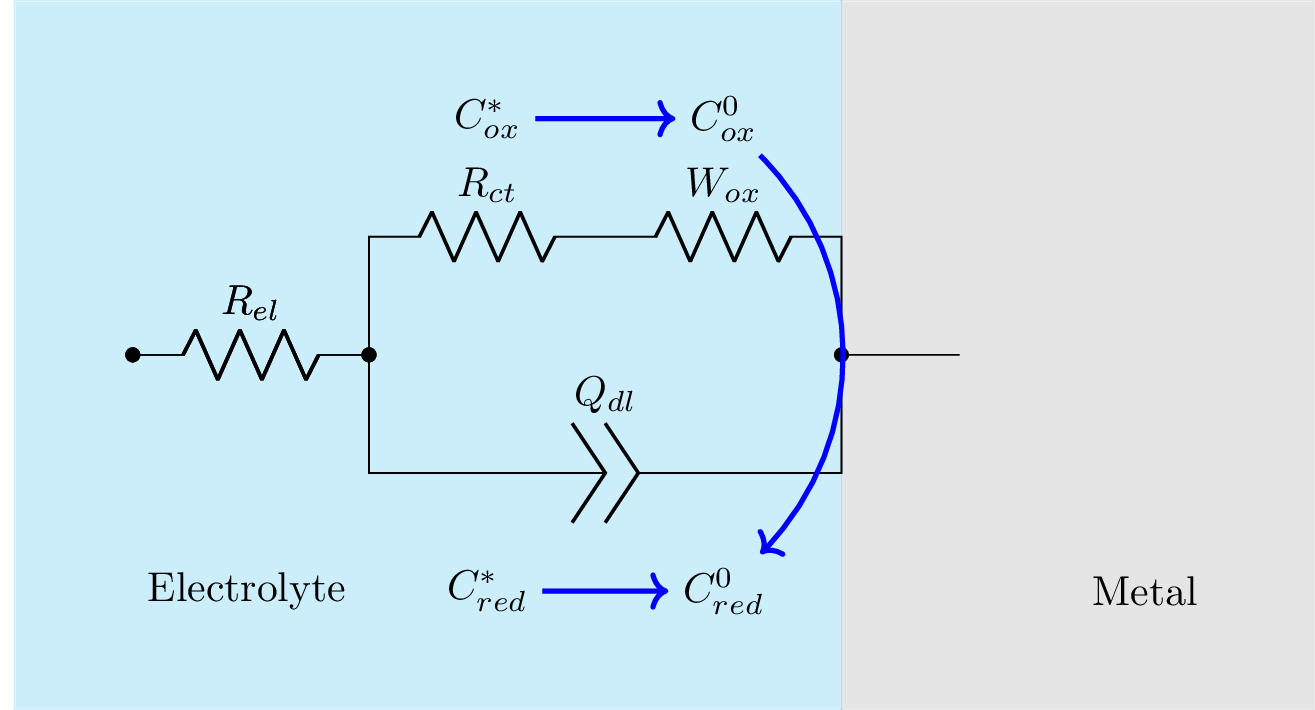
\includegraphics[width=\textwidth]{EIS-circuit-randles}
            \column{0.5\textwidth}
                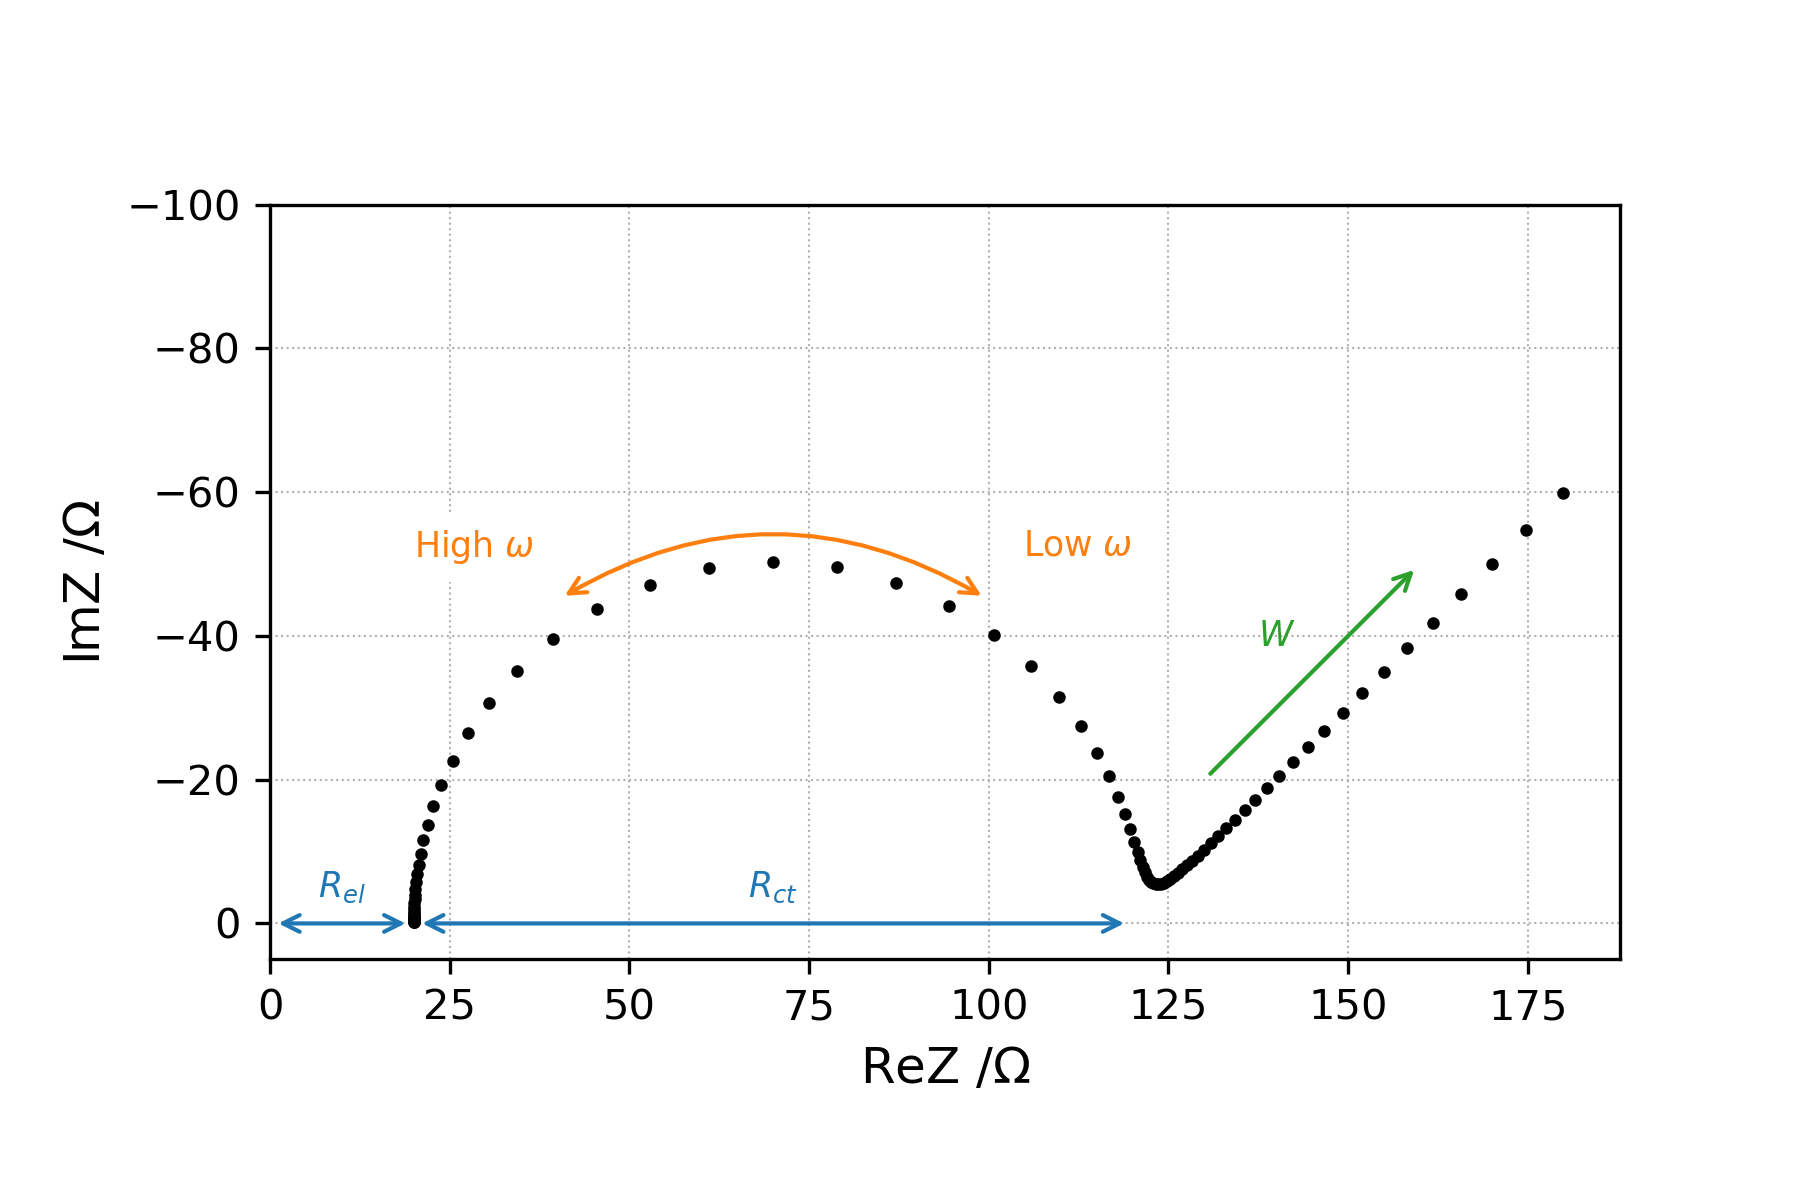
\includegraphics[width=\textwidth]{EIS-example-randles}
        \end{columns}
        
    \end{frame}

\section{Applications}
    \subsection{Electrolyte conductivity}
    \begin{frame}{Conductivity vs Temperature}
        EIS can be used to estimate the electrolyte conductivity at different temperatures.

        A calibration step is necessary at room temperature in order 
        to define the cell constant: $\kappa = A/l$

        Electrolyte containing $0.2 \,mmol \cdot L^{-1}$ $LiOH$ and $63 \, mmol \cdot L^{-1}$ $H_3BO_3$.
        \begin{figure}
            \centering
            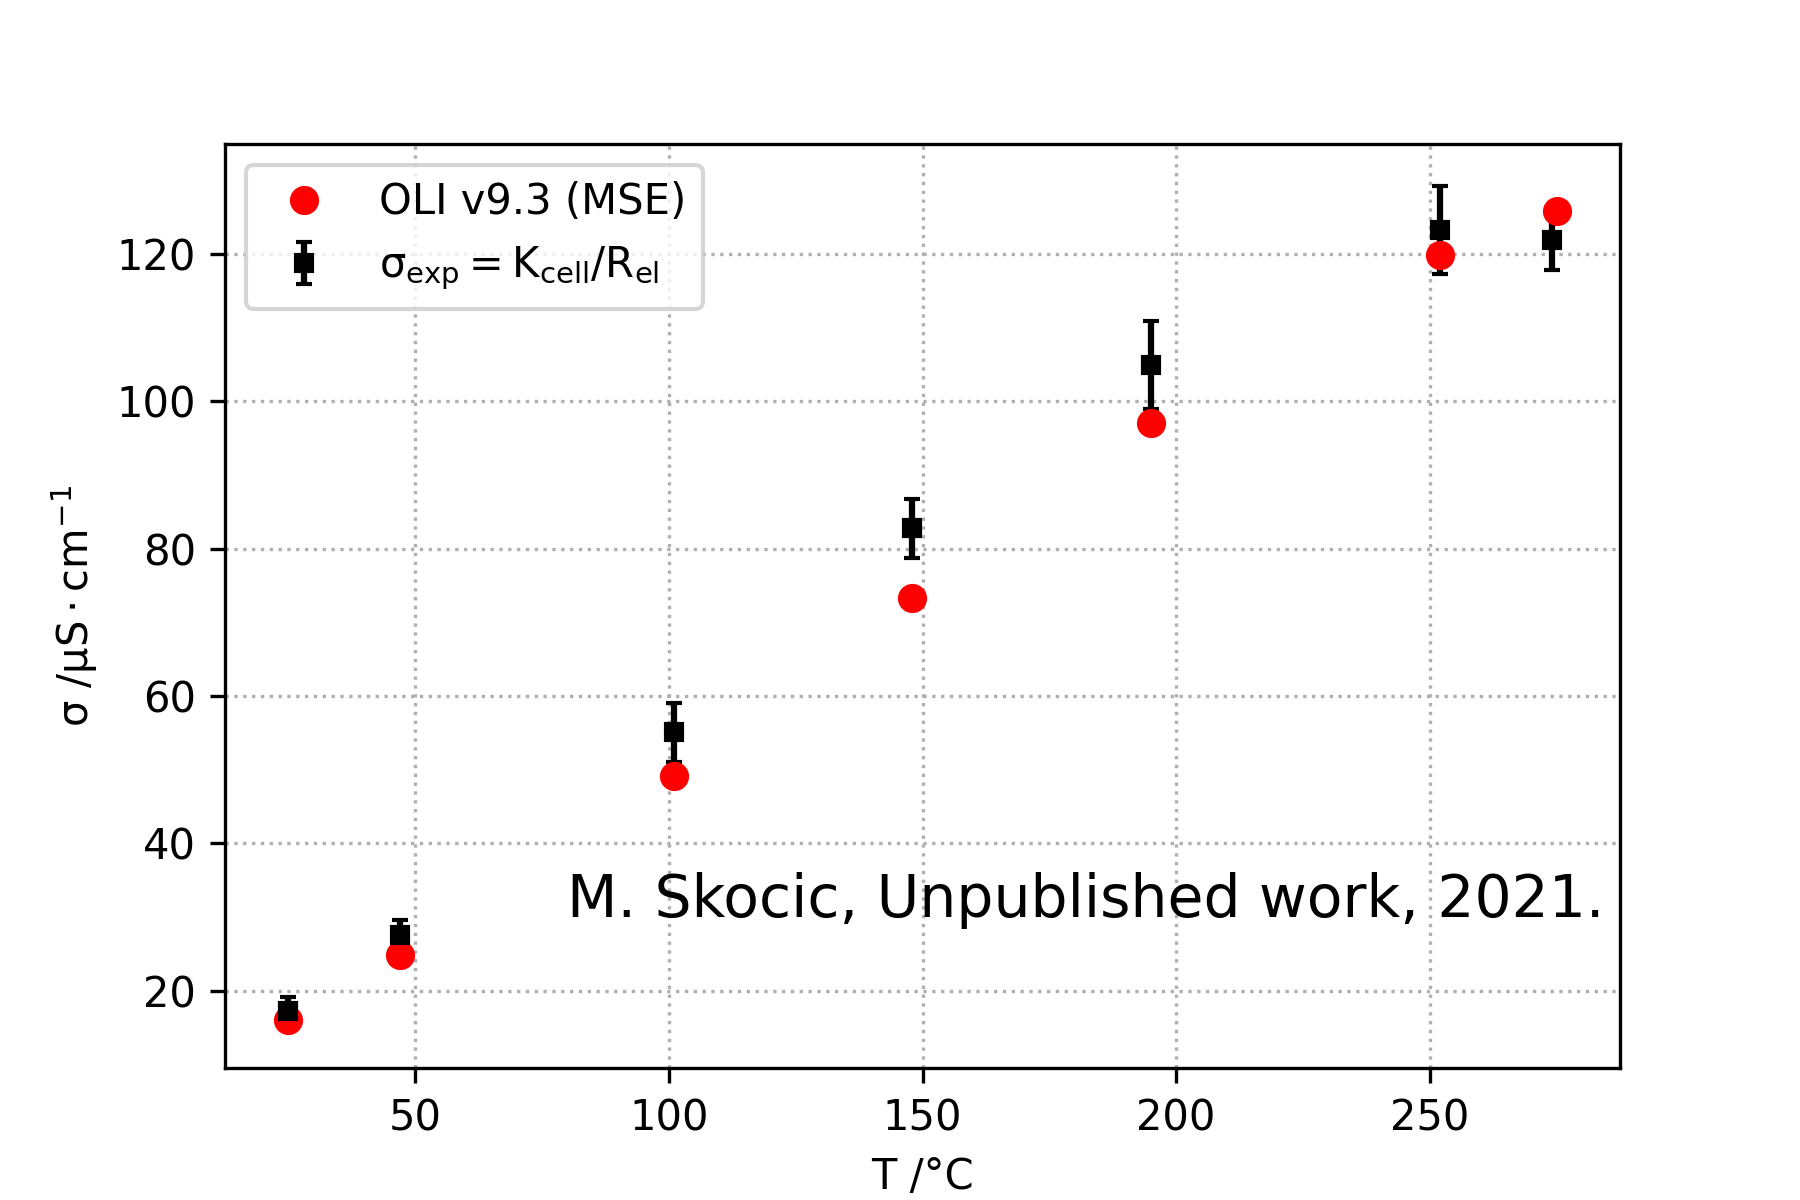
\includegraphics[width=0.65\textwidth]{EIS-application-conductivity}
        \end{figure}
    \end{frame}

    \subsection{Qualitative analysis}
    \begin{frame}{Corrosion mechanisms}
        2 domains are usually observed \citep{peyret2023}:
        \begin{itemize}
            \item  electronic contribution ($1Hz < f < 20 kHz$)
            \item  mass transfer contribution ($f \le 1Hz$)
        \end{itemize}
        Relative amplitude of both contributions vary according to the limiting corrosion mechanism.

        \begin{figure}
            \centering
            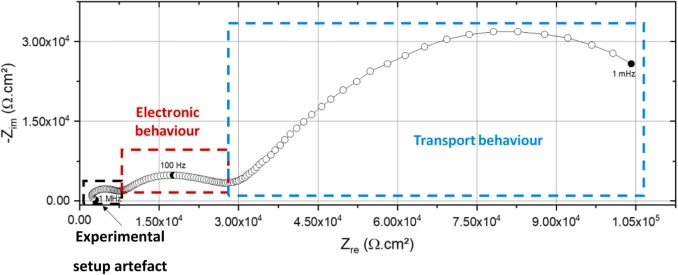
\includegraphics[width=0.65\textwidth]{EIS-application-contributions-peyret}
        \end{figure}
    \end{frame}

    \subsection{Quantitative Analysis} 
    \begin{frame}{Equivalent Circuit}
        For alloy forming passive layers, the diffusion in the electrolyte 
        is much faster than in the oxide.
        
        The limiting processes, most of the time, occur in the oxide layer
        \begin{itemize}
            \item  electronic contribution
            \item  mass transfer contribution
        \end{itemize}
        
        \begin{columns}
            \column{0.5\textwidth}
                \begin{figure}
                    \centering
                    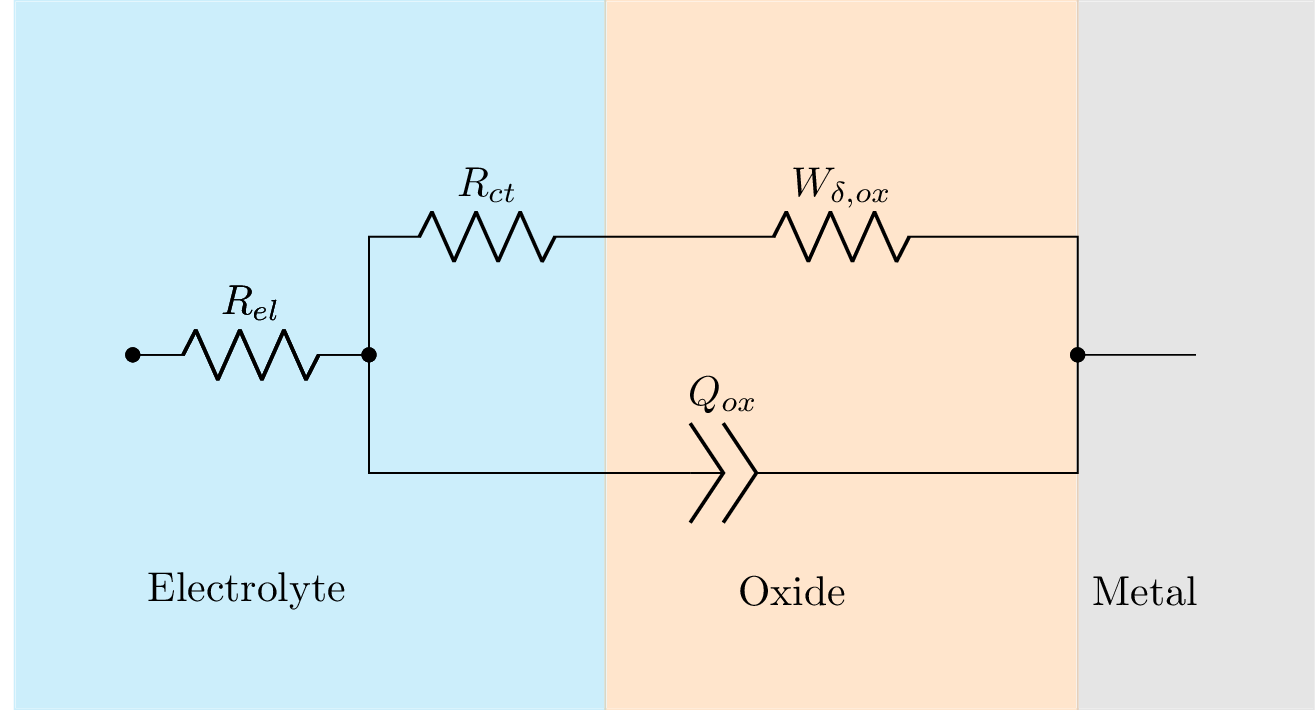
\includegraphics[width=\textwidth]{EIS-circuit-randles-flw}
                \end{figure}
            \column{0.5\textwidth}
                \centering
                \begin{figure}
                    \centering
                    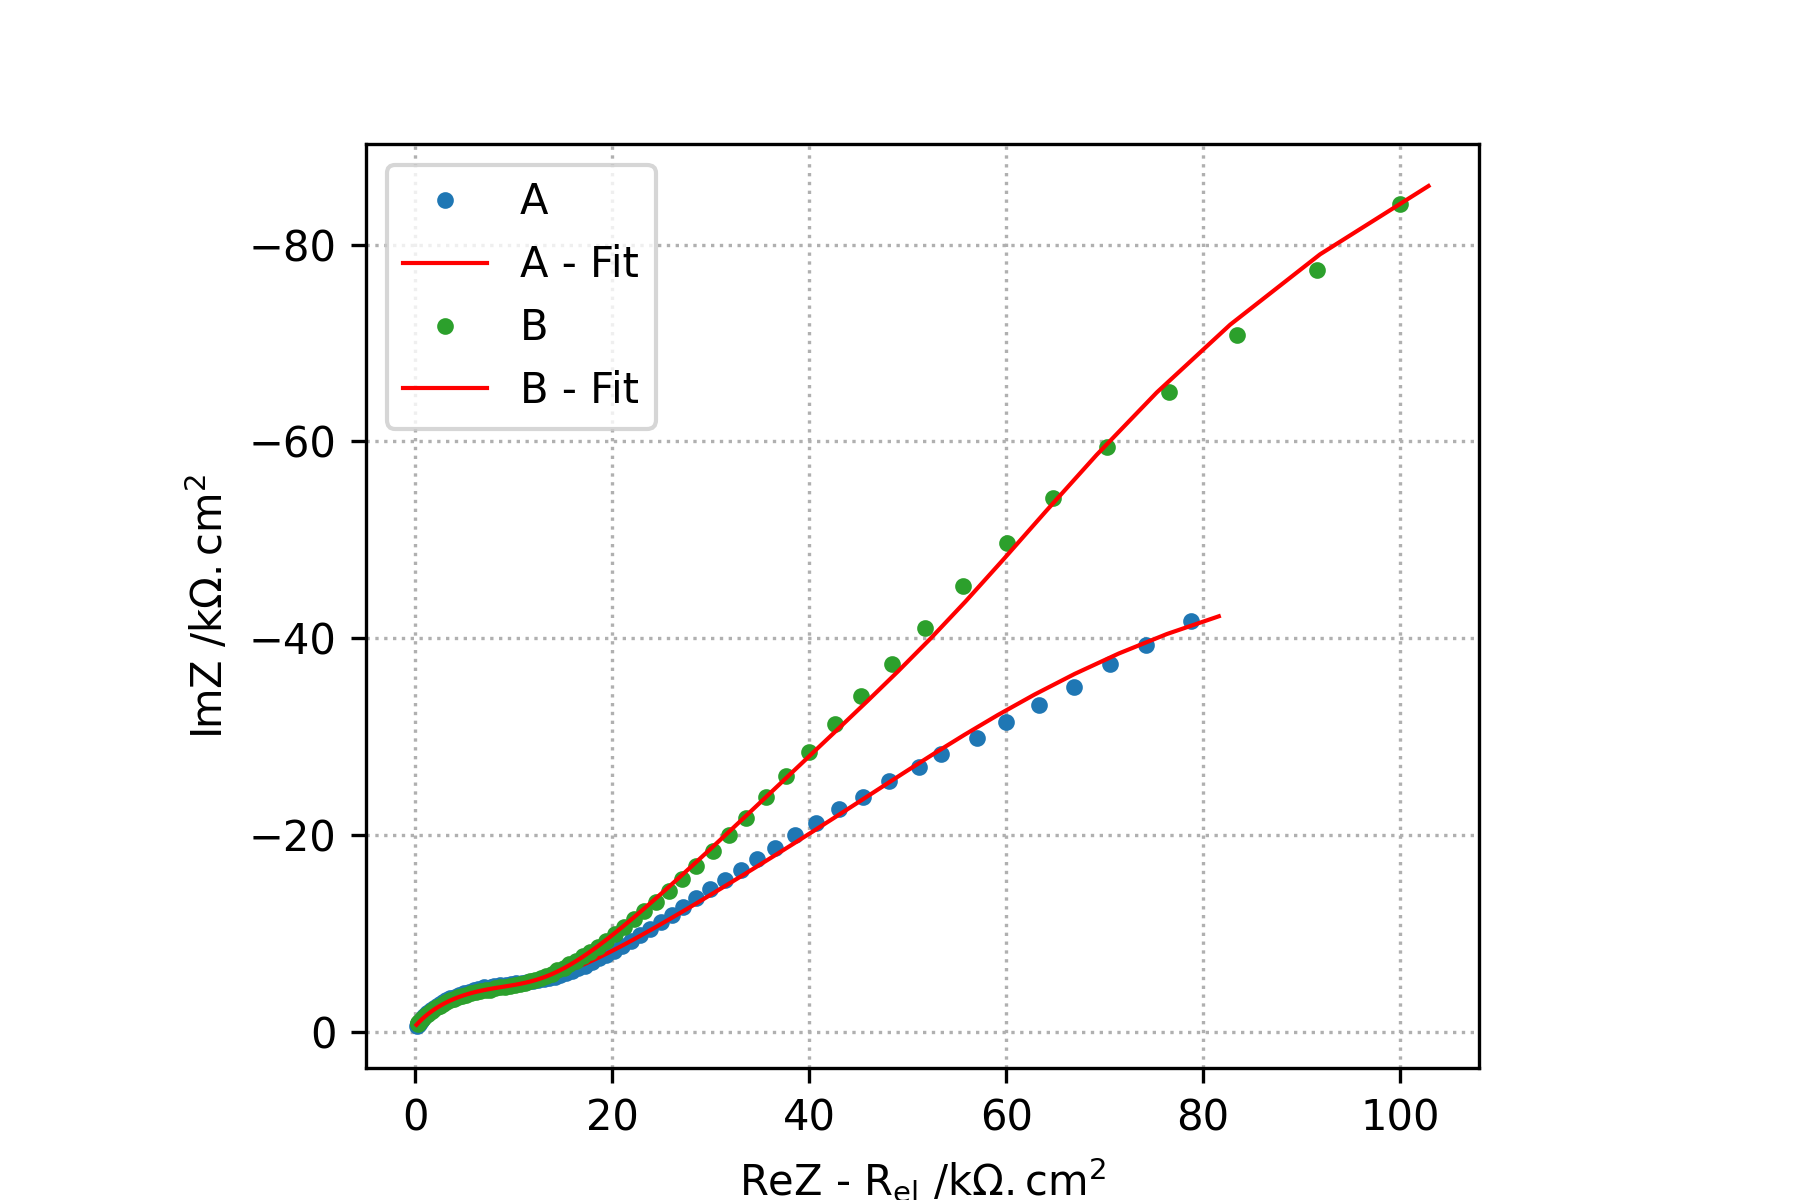
\includegraphics[width=\textwidth]{EIS-application-fit}
                \end{figure}
                \tiny M. Skocic, unpublished work, 2020.
        \end{columns}
    \end{frame}

    \begin{frame}{Numerical Fitting}
        Numerical fitting using CNLS (Complex Nonlinear Least Squares) allows 
        to determine the values of the electrochemical parameters for each circuit element \citep{boukamp1986}.

        Parameters such as effective capacitance, oxide thickness and diffusion coefficient can be computed.
        \vfill
        \begin{columns}
            \column{0.5\textwidth}
            \tiny
            \begin{tabular}{lll}
                \toprule
                Name                               & A                 & B               \\ \midrule
                $R_{el}$                           & $31 \pm 1$        & $99 \pm 2$      \\
                $R_{ct}$                           & $190 \pm 20$      & $280 \pm 2$     \\
                $W$                                & $3000 \pm 400$    & $5000 \pm 300$  \\
                $n$                                & $0.36 \pm 0.01$   & $0.49 \pm 0.01$ \\
                $\tau$                             & $120 \pm 40$      & $62 \pm 5$      \\
                $Q_{ox} \cdot 10^6 $               & $56 \pm 8$        & $102 \pm 8$     \\
                $a_{ox}$                           & $0.69 \pm 0.02$   & $0.60 \pm 0.01$ \\
                $\delta(\mu m)$                    & $0.10 \pm 0.03$   & $0.15 \pm 0.05$ \\
                $D \cdot 10^{12} (cm^2 \cdot s^{-1})$& $1.7 \pm 0.5$     & $1.9 \pm 0.9$   \\
                \bottomrule
            \end{tabular}
            \column{0.5\textwidth}
            \small
            $$ Z_{CPE}(\omega) = \frac{1}{Q(j\omega)^{\alpha}} $$
            $$ C = Q^{1/\alpha} \cdot R_{ct}^{\frac{\alpha - 1}{\alpha}} = \frac{\epsilon \epsilon _0 A}{\delta} $$
            $$ Z_{W_{\delta}}(\omega) = R_{\delta}\frac{\tanh \sqrt{(j\omega \tau)}}{\sqrt{j\omega \tau}} $$
            $$ \tau = \frac{\delta ^2}{D} $$
        \end{columns}
    \end{frame}

\section{Conclusion}
    \begin{frame}{Conclusions}
        \scriptsize
        EIS technique
            \begin{itemize}
                \item  EIS is a frequency domain electrochemical technique with small perturbations (linearization)
                \item  The circuit model represents the entire system
                \item  The objective is to build an optimal circuit model that is physically meaningful and minimizes the number of
                variables.
                \item  Evaluation of model with equivalent circuits and numerical fitting (CNLS)
            \end{itemize}

        Applications
            \begin{itemize}
                \item  Qualitative analysis of corrosion mechanism by observing the Nyquist plots for different alloys
                \item  Quantitative analysis for estimating the corrosion current densities
                \item  Quantitative analysis for computing physical parameters such as diffusion coefficients
                \item  Computation of electrolyte conductivity with respect to temperature
            \end{itemize}

        Difficulties
            \begin{itemize}
                \item  Noisy data at high temperature
                \item  Choice of the equivalent circuit
                \item  Propagation of errors on computed parameters
            \end{itemize}
    \end{frame}


% BIBLIOGRAPHY
\begin{frame}[allowframebreaks=0.9]{References}
\AtNextBibliography{\tiny}
%\nocite{*}
\printbibliography
\end{frame}

\end{document}
